\section{Experimentation}

\subsection{Strategy Hierarchy}
The following Hierarchy shows how we could organize Team behavior across 5 layers, from high-level strategy down to low-level execution. Each layer builds on the one above it, enabling modular, scalable control.

\begin{figure}[h]
    \centering
    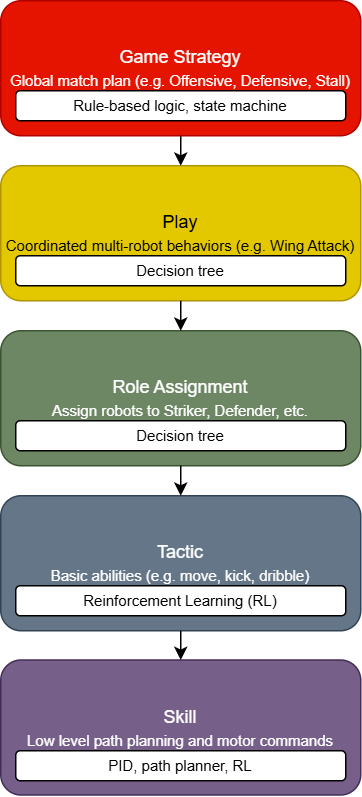
\includegraphics[width=0.8\linewidth]{../StrategyHierarchy.png}
    \caption{Hierarchical team behavior structure}
    \label{fig:strategy_hierarchy}
\end{figure}

\subsubsection{Game Strategy}
The top-layer defines the overall team behavior based on the given game state.
If we take Rule-based logic for example, we could look at time left to play and score.
Then if we are winning and the time is lower than a specified threshold, we could set the Strategy to Stall. This will then provide high-level context for all other decisions made below.

\subsubsection{Play}
The play layer selects coordinated maneuvers such as setting up a wing attack or forming a defensive wall. Selecting plays could be done by a decision tree based on factors like ball position, team formation, and opponent layout. Each play then sets constraints or goals for roles and tactics.

\subsubsection{Role Assignment}
This layer will dynamically assign robots to specific roles (e.g. striker, defender, goalie) based on their position, proximity to the ball, or other factors.
Optimization algorithms such as Hungarian matching have been used with great success.

\subsubsection{Tactic}
The tactic layer defines what action a robot should take in its current role.
This could be whether the robot should pass, dribble, shoot, or intercept.
This layer's decisions are highly context-sensitive and reinforcement learning is a good choice.

\subsubsection{Skill}
The skill layer handles the low-level physical execution of actions.
This could be moving to a position, kicking (how hard) or dribbling. Commonly used control methods are PID and path planning, but reinforcement learning can also be used to improve fine motor control, adaptability, or performance in unpredictable situations.
